\documentclass[aspectratio=169,11pt]{beamer}

\usetheme{Singapore}
\usepackage[utf8]{inputenc}
\usepackage{amsmath}
\usepackage{amsfonts}
\usepackage{amssymb}
\usepackage{graphicx}
\usepackage{hyperref}
\usepackage{booktabs}
\usepackage{listings}
\usepackage{xcolor}
\usepackage{caption}
\usepackage{subcaption}


% Define the settings for codechunks
\definecolor{codegreen}{rgb}{0,0.6,0}
\definecolor{codegray}{rgb}{0.5,0.5,0.5}
\definecolor{codepurple}{rgb}{0.58,0,0.82}
\definecolor{backcolour}{rgb}{0.9,0.9,0.9}
\lstdefinestyle{mystyle}{
    backgroundcolor=\color{backcolour},   
    commentstyle=\color{codegreen},
    keywordstyle=\color{magenta},
    numberstyle=\tiny\color{codegray},
    stringstyle=\color{codepurple},
    basicstyle=\ttfamily\footnotesize,
    breakatwhitespace=false,         
    breaklines=true,                 
    captionpos=b,                    
    keepspaces=true,                 
    numbers=left,                    
    numbersep=5pt,                  
    showspaces=false,                
    showstringspaces=false,
    showtabs=false,                  
    tabsize=2
}
\lstset{style=mystyle}

% Setup the bibliography
\usepackage[style=authortitle,backend=bibtex,citestyle=verbose]{biblatex}
\addbibresource{bibliography.bib}
\setbeamertemplate{bibliography item}[text]
\setbeamerfont{footnote}{size=\tiny}

% Allow footnotes with no number
\newcommand\blfootnote[1]{%
  \begingroup
  \renewcommand\thefootnote{}\footnote{#1}%
  \addtocounter{footnote}{-1}%
  \endgroup
}

% Allow section title slides
\AtBeginSection[]{
  \begin{frame}
  \vfill
  \centering
  \begin{beamercolorbox}[sep=8pt,center,shadow=true,rounded=true]{title}
    \usebeamerfont{title}\insertsectionhead\par%
  \end{beamercolorbox}
  \vfill
  \end{frame}
}

\author{Dr Stephen Pederson}
\title{Lecture 10: Single-Cell RNA Sequencing}
\subtitle{BIOINF3005/7160: Transcriptomics Applications}
%\setbeamercovered{transparent} 
\setbeamertemplate{navigation symbols}{} 
\logo{
	
\includegraphics[scale=0.3]{figures/UoA_logo_col_vert.png} 
} 
\institute{Bioinformatics Hub, \\The University of Adelaide} 
\date{May 25th, 2020} 
\subject{BIOINF3005/7160: Transcriptomics Applications} 


\begin{document}

\begin{frame}
\titlepage
\end{frame}

\begin{frame}
\footnotesize
\tableofcontents
\end{frame}


\section{Background}

\begin{frame}{Introduction}

	\begin{itemize}
		\item scRNA-Seq is the `latest and greatest' transcriptomic technique
		\item Previously all our analysis involved multiple cells per sample
		\item All were combined during tissue extraction, library preparation etc.
		\item Most experiments have \textbf{highly} heterogeneous cell populations, e.g.
		\pause
		\begin{itemize}
			\item Different regions of the brain contain highly specialised cells
			\item The immune system is highly complex
			\item Cancer samples have both infiltrating and tumour cells
		\end{itemize}
	\end{itemize}


\end{frame}

\begin{frame}{Introduction}

	\begin{itemize}
		\item If a gene is increased 2-fold in expression:
		\begin{itemize}
			\item Is this 2-fold in 100\% of cells?
			\item Or is it 4-fold in 50\% of cells?
			\item Or is it down 2-fold in 25\% and up 8-fold in 25\% and unchanged in 50\%?
		\end{itemize}
		\item Changes in gene expression can be highly specific to individual cell-types
		\item In general, determining heterogeneity of our samples is challenging
	\end{itemize}

\end{frame}

\begin{frame}{Introduction}

	\begin{itemize}
		\item The most intuitive solution is to obtain RNA from each cell and sequence
		\item Reality is much trickier than this
		\pause
		\item How do we characterise which cell is which cell-type?
		\item How do we capture as many transcripts from each cell as we can?
		\begin{itemize}
			\item Missing values are a huge issue in scRNA-seq
		\end{itemize}
		\item How do we compare within the same cell-types between experimental groups?
		\begin{itemize}
			\item E.g., treated and untreated cell types may not be assigned to the same cluster/cell-type
		\end{itemize}
	\end{itemize}

\end{frame}


\begin{frame}{Workflow Outline}

	\begin{center}
	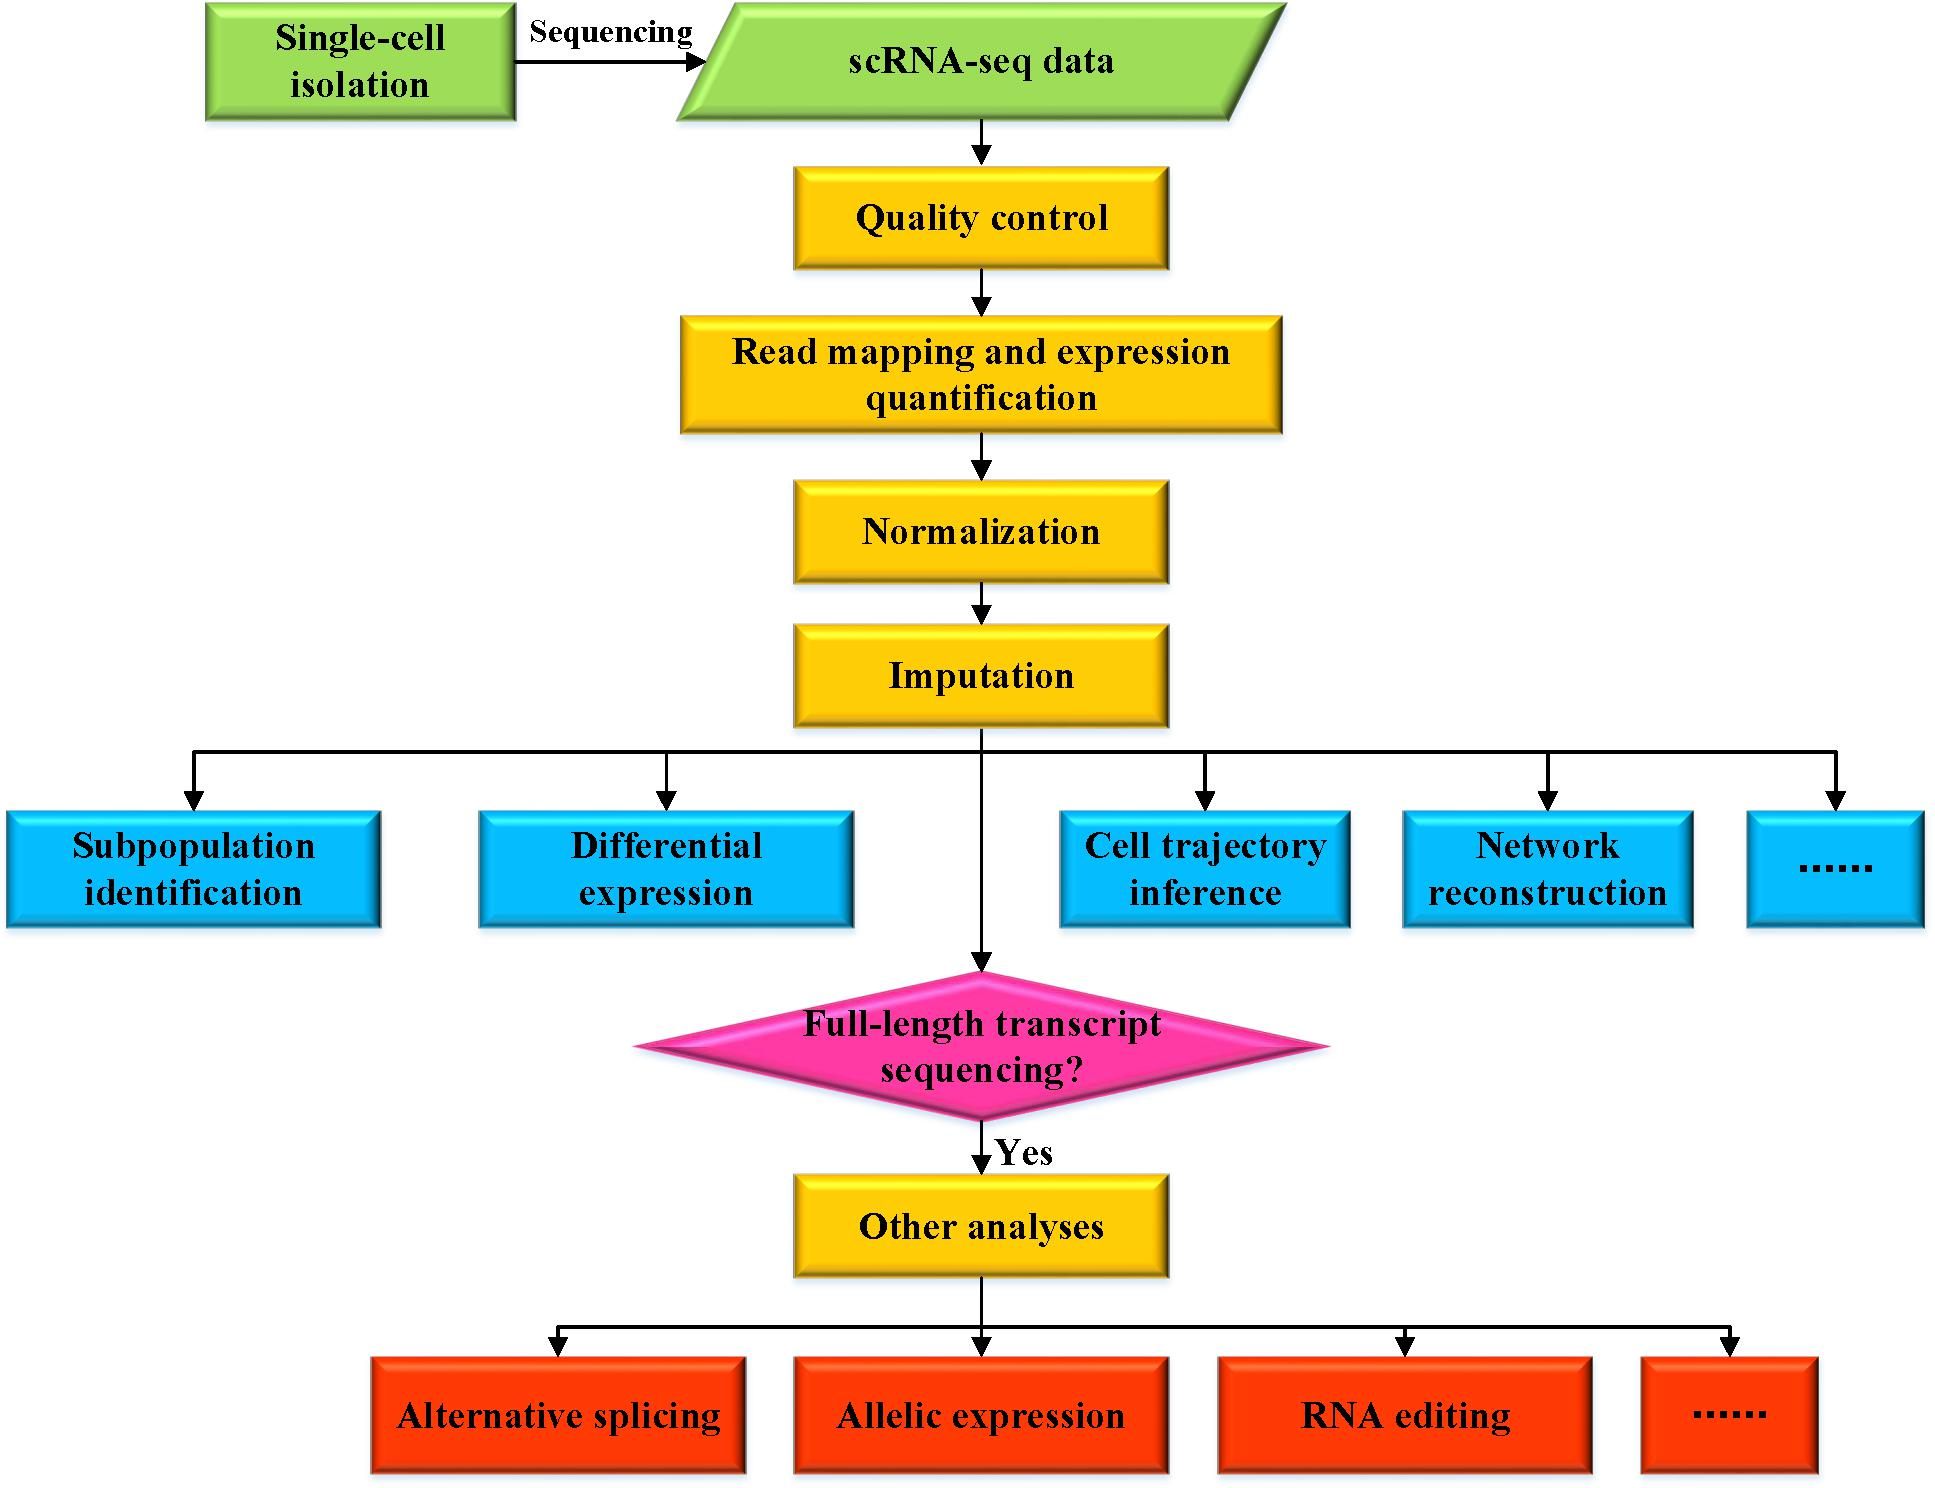
\includegraphics[width=0.5\textwidth]{figures/scRNAWorkflow.jpg} 
	\end{center}
	
	\blfootnote{Taken from \cite{10.3389/fgene.2019.00317}}

\end{frame}

\section{scRNA Protocols}

\begin{frame}{Isolating Individual Cells}

	\begin{itemize}
		\item Early protocols used a dilution series or manual isolation with a microscope (\textit{micromanipulation})
		\item Laser Capture Micro-dissection (LCM)
		\item Fluorescence-Activated Cell Sorting (FACS)
		\begin{itemize}
			\item Labelled antibodies to specific surface markers 
			\item MACS is a magnetic-based approach
		\end{itemize}
		\item Microfluidics/Droplet-based approaches
	\end{itemize}

\end{frame}

\begin{frame}{Protocol Timeline}

	\begin{center}
		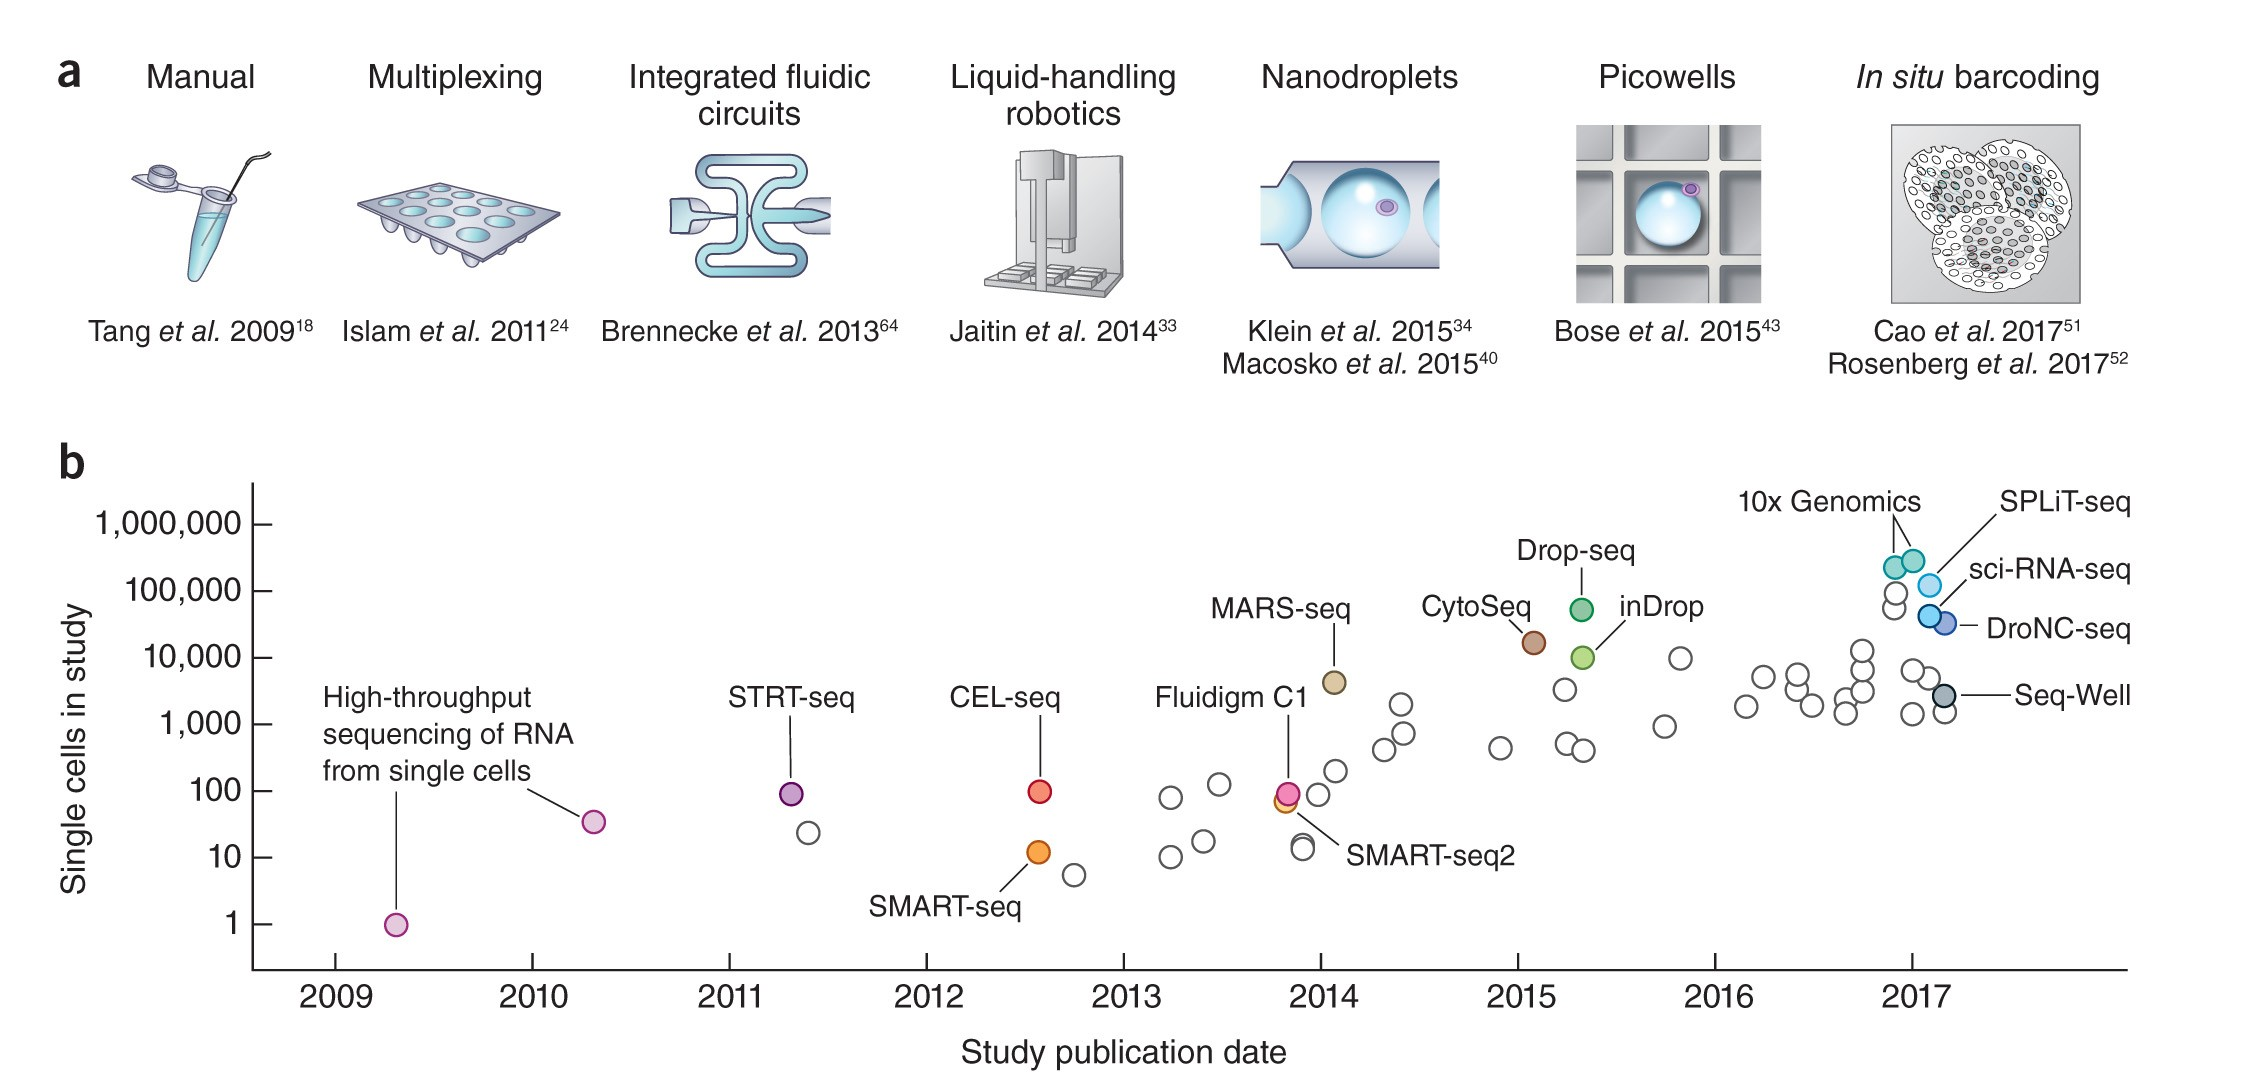
\includegraphics[width=0.8\textwidth]{figures/scRNATimeline.jpg} 
	\end{center}

	\blfootnote{Taken from \cite{pmid29494575}}

\end{frame}

\begin{frame}{Droplet-based Approaches}

	\begin{center}
		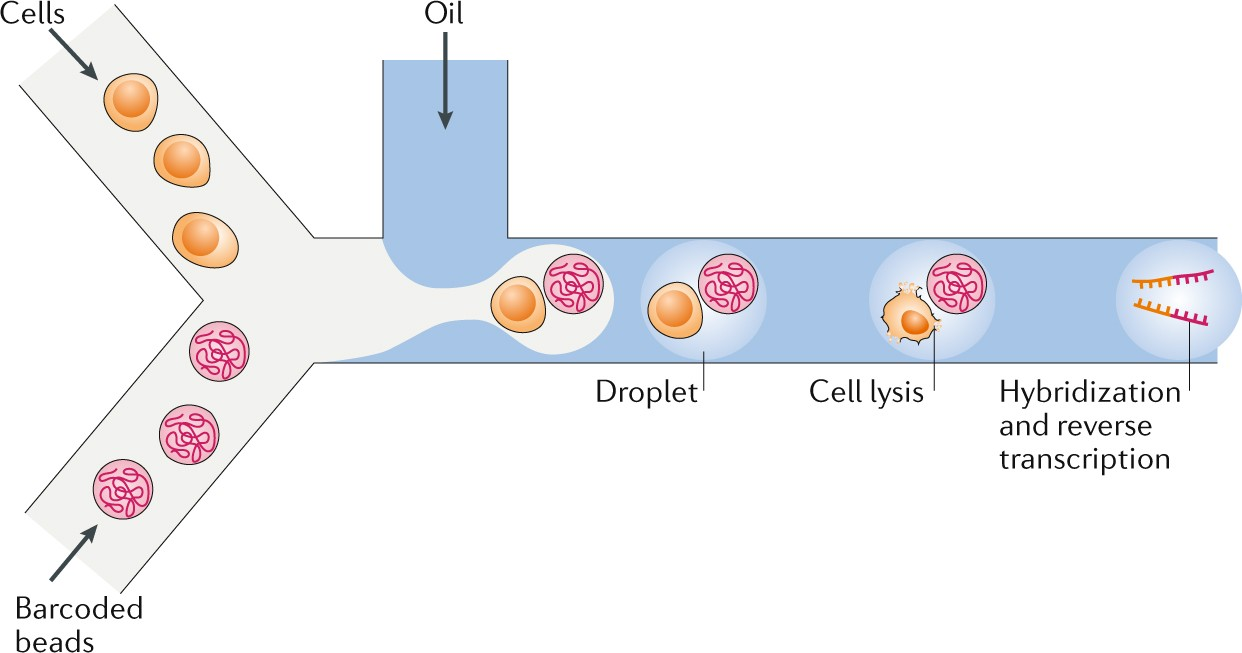
\includegraphics[width=0.7\textwidth]{figures/Droplet.jpg}
	\end{center}
	
	\blfootnote{Taken from \cite{pmid29789704}}

\end{frame}

\section{Data Analysis}

\subsection{QC}

\subsection{Quantification}

\subsection{Normalisation}

\subsection{Clustering}

\subsection{DE Analysis}

\subsection{Trajectory Analysis}

\section{Spatial Transcriptomics}


\end{document}
